\chapter{Introduction}
\label{sec:introduction}

Since the invention of modern computers, Monte Carlo methods have become an increasingly applied tool for challenging numerical problems in a wide variety of fields ranging from chemical physics to financial econometrics. Although the evolution of computers is proceeding, the complexity of considered problems is growing faster and Monte Carlo methods are now expected to deal with high dimensionalities and more and more complex structures. Hence the computational complexity of these methods is also nowadays a crucial question.

In this thesis we present a large subclass of Monte Carlo methods, the Markov chain Monte Carlo (MCMC) methods. The MCMC methodology~\autocite{Robert2005} provides a framework for many algorithms which affect the sampling from complex probability distributions in high dimensions by generating a Markov chain. It is therefore of interest to analyze the structure inherent in these algorithms to understand the computational complexity of MCMC methods. This is most naturally undertaken by studying the behavior of the method on a family of probability distributions indexed by a parameter and studying the cost of the algorithm as a function of that parameter. Therefore diffusion limits of MCMC methods in high dimensions provide a useful theoretical tool for studying computational complexity. In particular we will study these algorithms applied to a family of probability distributions found from finite-dimensional approximations of a measure on an infinite-dimensional space. This setting arises in widely used applications as Bayesian statistics or diffusion bridges.
Our interest is focused on Metropolis-Hastings MCMC methods. We study the random walk Metropolis algorithm (RWM) and the Metropolis-adjusted Langevin algorithm (MALA)~\autocite{Liu2004, Robert2005}. 

Consider a $ \pi^{N} $-invariant Metropolis Hastings–Markov chain $ \{ x^{k,N} \}_{k \geq 1} $, where $N$ denotes the dimension and $ \pi^{N} $ the target density. From the current state $ x $, we propose $ y $ drawn from the kernel $ q(x, y) $; this is then accepted with probability
\begin{equation}
\label{acceptance probability simple}
 \alpha^{N}(x,y)  := 1 \wedge \dfrac{\pi^{N}(y) q(y,x) }{\pi^{N}(x) q(x,y)}. .
\end{equation}

Two widely used proposals are the random walk proposal (obtained from
the discrete approximation of Brownian motion)
\begin{equation}
\label{RWM-proposals-simple}
  y = x + \sqrt{2\delta}\,Z^{N}, \qquad Z^{N} \thicksim \mathcal{N}\left( 0,I_N \right),
\end{equation}

and the Langevin proposal (obtained from the time discretization of the
Langevin diffusion)
\begin{equation}
\label{MALA-proposals-simple}
  y = x +  \delta \nabla \log \pi^{N} (x) + \sqrt{2\delta} Z^N, \qquad Z^{N} \thicksim \mathcal{N}\left( 0,I_N \right).
\end{equation}

Here $ 2 \delta $ is the proposal variance, a parameter quantifying the size of the discrete time increment; we will consider “local proposals” for which $ \delta $ is
small and note that $ \delta = \delta(N) $ will depend on the dimension $N$. The Markov chain corresponding to proposal (\ref{RWM-proposals-simple}) is the (RWM) algorithm~\autocite{Metropolis1953}, and the Markov transition rule constructed from the proposal (\ref{MALA-proposals-simple}) is known as the (MALA) algorithm~\autocite{Robert2005}.


\subsubsection*{Heuristic argument for an optimal scaling of MH methods}

In Figure~\ref{fig:3DscatterplotRWM}, the opitimal scaling characteristic of Metropolis-Hastings methods is illustrated by a Random Walk Metropolis-Hastings algorithm. The first 5000 samples produced by a RWM algorithm applied to a multimodal non-product target measure in dimension $N=10$ are depicted. Thereby every 1000 consecutive samples are labeled in the same color to better illustrate the movement of the generated chain. These sample chains generated by the RWM (or MALA) algorithm should ideally be not correlated (strong dependences in the samples leads to poorer MCMC estimates). Hence good mixture of the colors in Figure~\ref{fig:3DscatterplotRWM} visualizes fewer dependences between the samples and vice versa. 


\begin{figure}%[htb]
 \begin{center} 
  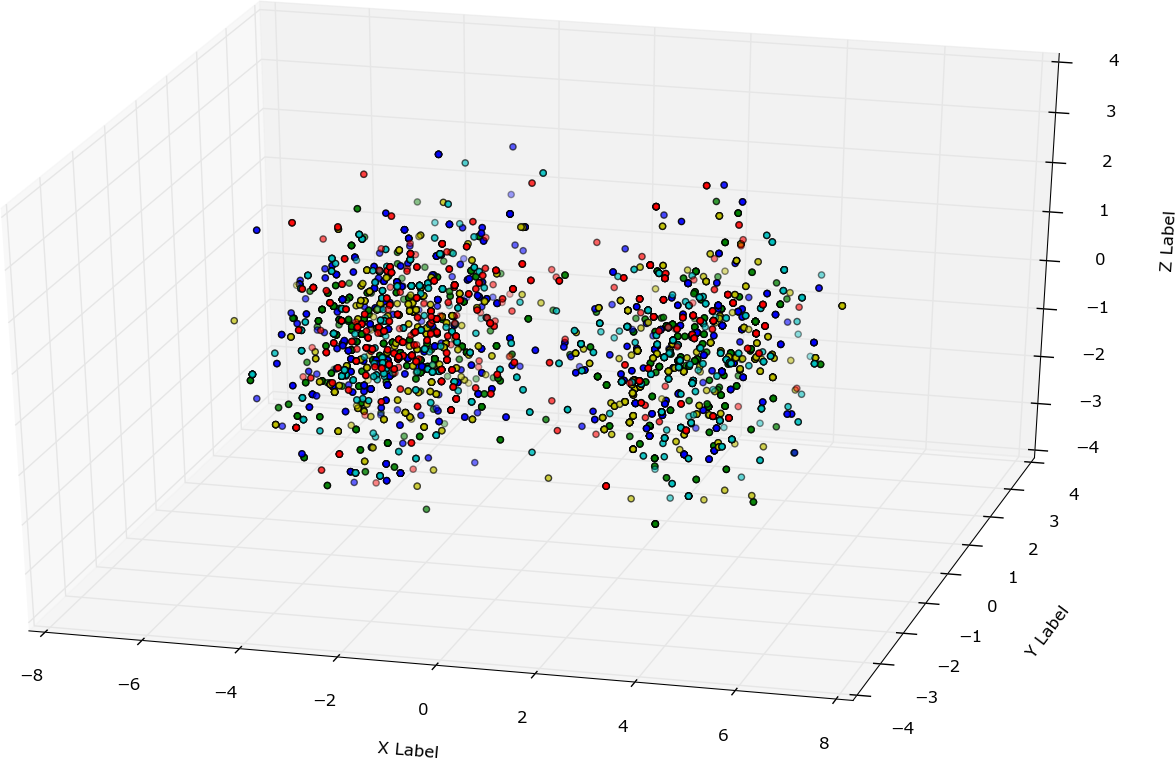
\includegraphics[width=0.6\textwidth]{figure_1}
  \vspace*{1mm}
  \subcaption{'Optimal scaled' RWM algorithm with a good mixing between both modes.}
  \label{fig:3DscatterplotRWM-optimal}
  \vspace*{3mm}
  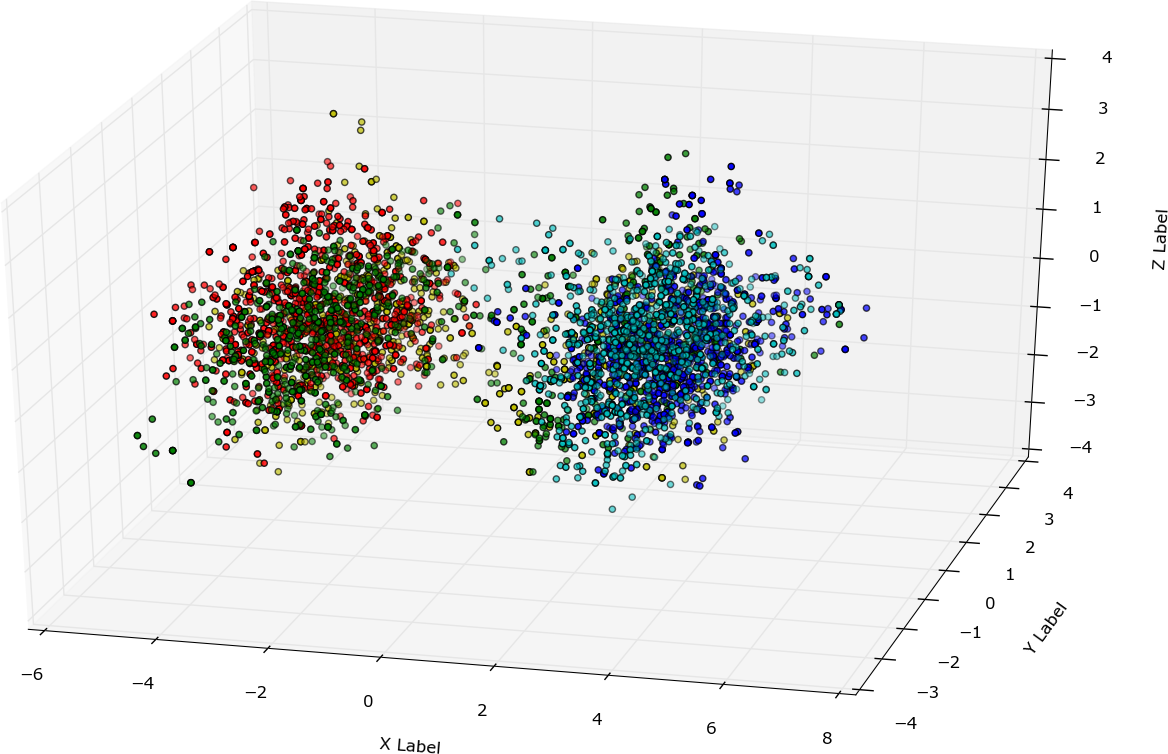
\includegraphics[width=0.6\textwidth]{figure_2}
  \vspace*{1mm}
  \subcaption{Too small proposal variance with strong dependences.}
  \vspace*{3mm}
  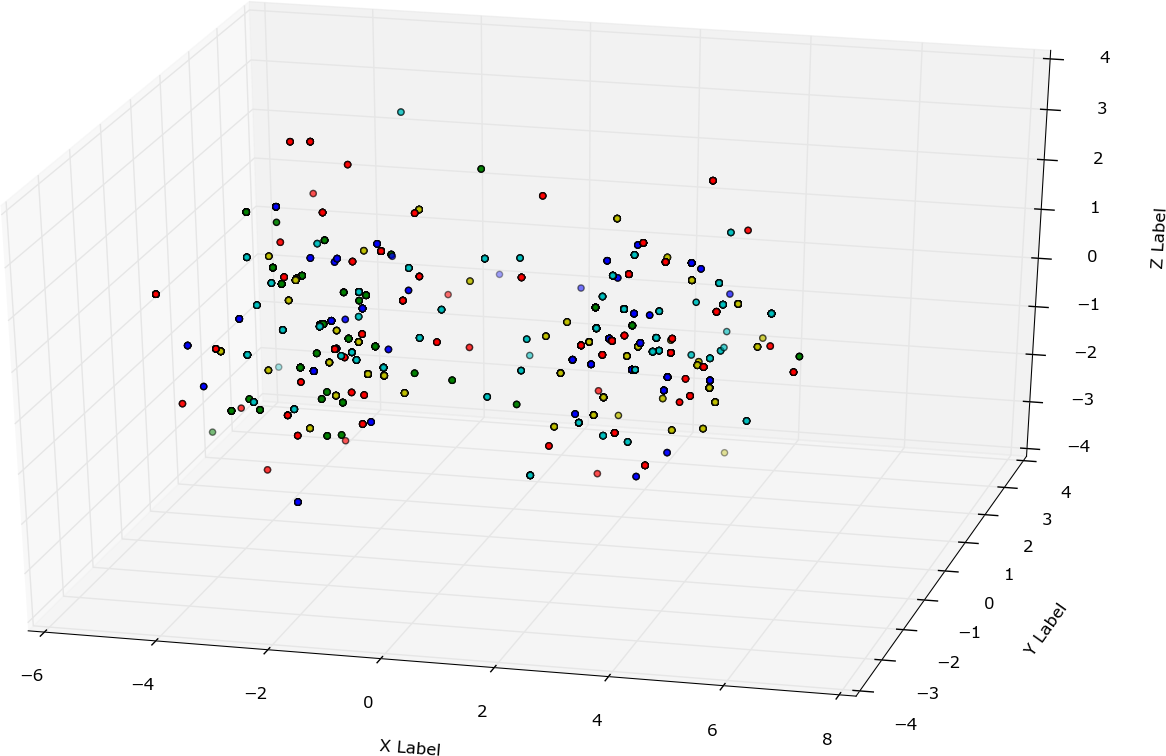
\includegraphics[width=0.6\textwidth]{figure_3}
  \vspace*{1mm}
  \subcaption{Too large proposal variance causes too much rejected movements.}
 \end{center}
  \caption{5000 samples produced by a RWM algorithm of a multimodal non-product target density. Every 1000 consecutive samples are labeled in the same color.}
  \label{fig:3DscatterplotRWM}
\end{figure}

A simple numerical simulation as in Figure~\ref{fig:3DscatterplotRWM} illustrates that too small or large proposal variances make the algorithm arbitrarily poor. For extremely small proposal variances, the algorithm will propose only small jumps and almost every step will be accepted. Therefore the average acceptance rate is almost one. However, the size of the proposed jumps is too small to explore the target distribution rapidely. The convergence of the algorithm to its stationary distribution will take too long. In the case of a too large proposal variances, the algorithm will propose large jumps (to far distant regions). It will therefore reject most of its proposed moves and the Markov chain stays very long in single states. Hence, it seems reasonable that there exist 'good' intermediate values for the proposal variance (see Figure~\ref{fig:3DscatterplotRWM-optimal}). This performance is for every dimension $N$ observable. Moreover, such 'optimal' intermediate proposal variances $ \delta(N) $ decrease with increasing dimension $N$.

\subsection*{Statement of the problem}

The above introduced structure of Metropolis-Hastings methods is rather simple. At each step a move is proposed according to~(\ref{RWM-proposals-simple}) or~(\ref{MALA-proposals-simple}) and this candidate is accepted with a certain probability~(\ref{acceptance probability simple}). These quantities depend on the target distribution $ \pi^{N} $ and the proposal kernel $ q(x,y) $, which is characterized by the proposal variance $ \delta(N) $ in the case of Gaussian jumps. Hence all occurring quantities can be indexed by a parameter; in this case the dimension $N$. Our aim is to study the cost as a function of dimension for the RWM and MALA algorithm applied to different families of probability distributions. Early results~\autocite{Roberts1997, Roberts1998} concerned product measures for wich an optimal scaling via diffusion limits for RWM and MALA was obtained. It was shown that the computational comlexity of RWM started in stationarity and applied to simple product distributions is $\mathcal{O}(N)$ for an average acceptance rate of 0.234~\autocite{Roberts1997}. Similarly, the cost of MALA, started in stationarity and applied to simple product distributions was characterized by $\mathcal{O}(N^{1/3})$ for an average acceptance rate of 0.573~\autocite{Roberts1998}. In this work, we want to resume the results of Mattingly, Pillai and Stuart~\autocite{Mattingly2010} and Pillai, Stuart and Thi\'{e}ry~\autocite{Pillai2012}. They succeeded to prove that the optimal scaling of RWM and MALA as mentioned above holds for finite-dimensional approximations of measures obtained from Gaussian measures in infinte-dimensional Hilbert spaces by a change of measures. This specific setting occurs in widely used applications as Bayesian statistics and diffusion bridges.

More precisely, we will prove a diffusion limit result for RWM and MALA in the above Hilbert space setting, where the speed of the interpolant of the generated Markov chains and the proposal variance of the RWM or MALA candidates scales in the correct sense. This diffusion limit result provides us to quantify the computational cost or efficiency uniquely but on the other hand this statement holds only asymptotically.




\subsection*{Own contributions}

My contributions to the present topic.
\begin{itemize}
 \item Combining and resuming the proof (strategy) of Mattingly, Pillai and Stuart~\autocite{Mattingly2010} and Pillai, Stuart and Thi\'{e}ry~\autocite{Pillai2012}.
 \item Give a comprehensive overview.
 \item Numerical studies.
\end{itemize}


\subsection*{Outline}

A brief outline of the structure of this work.


\subsection*{Acknowledgements}

A list of persons, who deserve my acknowledgements: advisor, parents, friends.



